\documentclass[12pt]{exam}

% essential packages
\usepackage{fullpage} % margin formatting
\usepackage{enumitem} % configure enumerate and itemize
\usepackage{amsmath, amsfonts, amssymb, mathtools} % math symbols
\usepackage{xcolor, colortbl} % colors, including in tables
\usepackage{makecell} % thicker \Xhline in table
\usepackage{graphicx} % images, resizing

% sometimes needed packages
\usepackage{hyperref} % hyperlinks
\usepackage{tikz} % drawing graphs

% paragraph formatting
\setlength{\parskip}{6pt}
\setlength{\parindent}{0cm}

% newline after Solution:
\renewcommand{\solutiontitle}{\noindent\textbf{Solution:}\par\noindent}

% less space before itemize/enumerate
\setlist{topsep=0pt}

% creates \filcl to grey out cells for groupwork grading
\newcommand{\filcl}{\cellcolor{gray!25}}

% creates \probnum to get the problem number
\newcounter{probnumcount}
\setcounter{probnumcount}{1}
\newcommand{\probnum}{\arabic{probnumcount}. \addtocounter{probnumcount}{1}}

% use roman numerals by default
\setlist[enumerate]{label={(\roman*)}}

% creates custom list environments for grading guidelines, question parts
\newlist{guidelines}{itemize}{1}
\setlist[guidelines]{label={}, left=0pt .. \parindent, nosep}
\newlist{gwguidelines}{enumerate}{1}
\setlist[gwguidelines]{label={(\roman*)}, nosep}
\newlist{qparts}{enumerate}{2}
\setlist[qparts]{label={(\alph*)}}
\newlist{qsubparts}{enumerate}{2}
\setlist[qsubparts]{label={(\roman*)}}
\newlist{stmts}{enumerate}{1}
\setlist[stmts]{label={(\roman*)}, nosep}
\newlist{pflist}{itemize}{4}
\setlist[pflist]{label={$\bullet$}, nosep}
\newlist{enumpflist}{enumerate}{4}
\setlist[enumpflist]{label={(\arabic*)}, nosep}

\printanswers

\newcommand{\prevhwnum}{6}
\newcommand{\hwnum}{7}

\begin{document}
%%%%%%%%%%%%%%% TITLE PAGE %%%%%%%%%%%%%%%
\title{EECS 203: Discrete Mathematics\\
  Winter 2024\\
  Homework \hwnum{}}
\date{}
\author{}
\maketitle
\vspace{-50pt}
\begin{center}
  \huge Due \textbf{Thursday, Mar. 21}, 10:00 pm\\
\Large No late homework accepted past midnight.\\
\vspace{10pt}
\large Number of Problems: $8+2$
\hspace{3cm}
Total Points: $100+18$
\end{center}
\vspace{25pt}
\begin{itemize}
    \item \textbf{Match your pages!} Your submission time is when you upload the file, so the time you take to match pages doesn't count against you.
    \item Submit this assignment (and any regrade requests later) on Gradescope. 
    \item Justify your answers and show your work (unless a question says otherwise).
    \item By submitting this homework, you agree that you are in compliance with the Engineering Honor Code and the Course Policies for 203, and that you are submitting your own work.
    \item Check the syllabus for full details.
\end{itemize}
\newpage
%%%%%%%%%%%%%%% TITLE PAGE %%%%%%%%%%%%%%% 

\section*{Individual Portion}

\subsection*{\probnum Growing your Growth Mindset [5 points]}

\begin{qparts}
    \item Watch the linked video about developing a growth mindset. This is a different video than the one you saw in lecture.
    \item Rewrite the last two fixed mindset statements as growth mindset statements.
    \item Write down one of your recurring fixed mindset thoughts, then write a thought you can replace it with that reflects a growth mindset.
\end{qparts}

\textbf{Video:} \href{https://tinyurl.com/eecs203growthMindset}{Developing a Growth Mindset (tinyurl.com/eecs203growthMindset)}

\textbf{What to submit:} Your three pairs of fixed and growth mindset statements 
(the two from the table, and one that you came up with on your own).

\begin{center}
\begin{tabular}{ |p{18em}|p{18em}| } 
\hline
\textbf{Fixed Mindset Statement} & \textbf{Growth Mindset Statement}\\
\hline

When I have to ask for help or get called on in lecture, I get anxious and feel like people will think I’m not smart.

& The question I have is likely the same question someone else in lecture may have. It’s important for me to ask so I can better understand what I am learning.
\\ \hline

I’m jealous of other people’s success.

& I am inspired and encouraged by other people’s success. They show me what is possible.

\\ \hline

I didn’t score as high on the exam as I expected. I’m not going to do well in this class and should drop it.

& I learned from my mistakes on exam 1, and exam 2 will be a new opportunity for me to practice what I’ve learned.

\\ \hline

This class is hard for me, so I am not fit for this major.
& [FILL IN YOUR OWN]
\\ \hline

Either I'm good at Discrete Math, or I'm not. 
& [FILL IN YOUR OWN]
\\ \hline

[FILL IN YOUR OWN] & [FILL IN YOUR OWN] \\ 
\hline
\end{tabular}
\end{center}

\begin{solution}
Any growth mindset version of the fixed mindset statements is ``correct.'' Similarly, for the ``choose your own'' pair of statements, any fixed mindset statement that you've converted to a growth mindset statement works. We've included some example statements below.

\begin{center}
\begin{tabular}{ |p{15em}|p{15em}| } 
\hline
\textbf{Fixed Mindset Statement} & \textbf{Growth Mindset Statement}
\\ \hline

This class is hard for me, so I am not fit for this major.

&\textbf{Example: This class is hard for me. The skills I am learning as I work to meet the challenge will serve me well throughout the rest of this major. }

\\ \hline

Either I'm good at Discrete Math, or I'm not.

& \textbf{Example: There are concepts in this class that I do not feel comfortable with \textit{yet}. I can work to improve my understanding with practice, by asking questions in discussion, and by going to office hours to clear up areas of uncertainty. }

\\ \hline

\textbf{Example: I'm just not an organized person. }

& \textbf{Example: I've had a hard time staying organized in the past. I can find resources and ideas for keeping organized and try a few to decide which ones work best for me. }

\\ \hline
\end{tabular}
\end{center}

\textbf{Grading Guidelines [5 points]}
\begin{guidelines}
    \item +5 valid growth mindset statements
\end{guidelines}
\end{solution}

\subsection*{\probnum Sketchy Compositions [15 points]}
Consider $f \colon X \to Y $ and $g \colon Y \to X$. \textbf{Prove or disprove} each of the following statements.

\begin{qparts}
    \item If  $ f \circ g $ is one-to-one, then $ g $ must be one-to-one.
    \item If $ g \circ f $ is one-to-one, then $ g $ must be one-to-one.
\end{qparts}

\begin{solution}
\begin{qparts}
    \item
    \textbf
    {Solution 1:}

    We shall prove this statement with a proof by contradiction.

    Assume the negation of the statement: $f$ and $f\circ g$ are one-to-one and $g$ is not one-to-one. If $g$ is not one-to-one, there must exist some $y_{1}, y_{2} \in Y$ such that $y_{1}\neq y_{2}$ but $g(y_{1})=g(y_{2})$. Both $g(y_{1})$ and $g(y_{2})$ exist in $X$, so we can apply the function $f$ to both sides to get $f(g(y_1))=f(g(y_2))$. Since we have $f(g(y_1))=f(g(y_2))$ for $y_1 \neq y_2$, $f \circ g$ is not one-to-one. This contradicts our original assumption that $f\circ g$ is one-to-one. Therefore, $g$ must also be one-to-one.
    
    \textbf{Solution 2:}
    We will prove that $g$ is one-to-one directly.
    
    Let $y_1, y_2 \in Y$. Consider $g(y_1) = g(y_2)$. Both $g(y_{1})$ and $g(y_{2})$ exist in $X$, so we can apply the function $f$ to both sides to get $f(g(y_1)) = f(g(y_2))$. This is equivalent to $(f \circ g)(y_1) = (f \circ g)(y_2)$. Since $f \circ g$ is one-to-one, $y_1 = y_2$. Thus, $g$ is one-to-one.

    \item
    We shall disprove this statement.

    Consider the following scenario where $X = \{a, b, c\}$ and $Y = \{1, 2, 3, 4\}$. Let $f$ be the function such that $f(a) = 1, f(b) = 2$ and $f(c) = 3$. Let $g$ be the function such that $g(1) = a, g(2) = b, g(3) = c,$ and $g(4) = c$. Since $g(3) = c = g(4)$ but $3 \neq 4$, $g$ is \textbf{not} one-to-one. Therefore, $g \circ f$ is the function such that $(g \circ f)(a) = a, (g \circ f)(b) = b,$ and $(g \circ f)(c) = c$. $g \circ f$ is one-to-one.
    
    Since our example shows a situation where $T \to F$, the original statement is false in this situation. Since we have shown a counter example, this original statement is false.
\end{qparts}

\textbf{Draft Grading Guidelines [15 points]}

\textbf{Part a (contradiction):}
\begin{guidelines}
    \item +1 chooses to prove
    \item +2 correct assumption for a proof by contradiction
    \item +2 uses the definition of one-to-one to find elements in the domain of $g$ such that $y_1 \ne y_2$ but $g(y_1) = g(y_2)$
    \item +2 applies $f$ to both sides (must not say it is due to $f$ being one-to-one)
    \item +1 arrives at a contradiction and concludes that $g$ is one-to-one
\end{guidelines}
\textbf{Part a (direct):}
\begin{guidelines}
    \item +1 chooses to prove
    \item +2 takes arbitrary $y_1$ and $y_2$ in the domain of $g$ and assumes $g(y_1) = g(y_2)$
    \item +2 plugs both sides into $f$
    \item +1 notes $f(g(y)) = (f \circ g)(y)$
    \item +2 applies the definition of one-to-one to conclude $y_1 = y_2$
\end{guidelines}
\textbf{Part b:}
\begin{guidelines}
    \item +1 chooses to disprove
    \item +2 provides a correct counterexample
    \item +2 correctly argues that $g$ is not one-to-one
    \item +2 correctly argues that $g \circ f$  one-to-one
\end{guidelines}
\end{solution}

\subsection*{\probnum Flippy Function Fun! [15 points]}

A function $f\colon A\to A$ is said to be \textit{flippy} if for all $a\in A,$ $f(f(a))=a.$ \textbf{Prove or disprove} each of the following statements

\begin{qparts}
    \item If $f\colon A\to A$ is flippy, then $f$ is bijective. (Either prove $f$ is both onto and one-to-one using their respective definitions, or provide a counterexample.)
    \item If $f\colon A\to A$ and $g\colon A\to A$ are flippy, then $f\circ g$ must be flippy.
\end{qparts}

\begin{solution}
What we call flippy functions are more commonly called \textit{involutions}. They have several interesting properties, including those proved here.

\begin{qparts}
    \item We will prove this statement:
    
    \textbf{Onto:} Let $y\in A.$ To show $f$ is onto, we must find an $x\in A$ such that $f(x)=y.$ Note that $f(y)\in A,$ and that by the definition of flippy, $f(f(y))=y.$ So we take $x=f(y),$ proving $f$ is onto.
    
    \textbf{One-to-one:} Let $x_1,x_2\in A$ and suppose $f(x_1)=f(x_2).$ Then $f(f(x_1))=f(f(x_2)),$ which implies $x_1=x_2$ by the definition of flippy. So $f$ is one-to-one.
    
    Since $f$ is onto and one-to-one, $f$ is bijective.
\end{qparts}
\begin{qparts}[resume]
    \item This not necessarily the case, so we need to \textbf{disprove}. As a counterexample, take $A=\{1,2,3\},$ and $f$ and $g$ defined as follows:
    \begin{align*}
        \begin{split}
        f(a)&=\begin{cases}
            2 & a=1 \\
            1 & a=2 \\
            3 & a=3
        \end{cases}
        \end{split}
        \begin{split}
        g(a)&=\begin{cases}
            1 & a=1 \\
            3 & a=2 \\
            2 & a=3
        \end{cases}
        \end{split}
    \end{align*}

    Now, we show that $f$ and $g$ are both flippy.
    \begin{align*}
        \begin{split}
            f(f(1)) &= f(2) = 1\\
            f(f(2)) &= f(1) = 2\\
            f(f(3)) &= f(3) = 3
        \end{split}
        \begin{split}
            g(g(1)) &= g(1) = 1\\
            g(g(2)) &= g(3) = 2\\
            g(g(3)) &= g(2) = 3
        \end{split}
    \end{align*}
    
    However, $f \circ g$ isn't flippy, because
    \begin{align*}
        (f\circ g)((f\circ g)(1)) &= f(g(f(g(1)))) \\
        &= f(g(f(1))) \\
        &= f(g(2)) \\
        &= f(3) \\
        &= 3\ne 1.
    \end{align*}
\end{qparts}

\textbf{Draft Grading Guidelines [15 points]}

\textbf{Part a:}
\begin{guidelines}
    \item +2 attempts to prove
    \item +1 says that $f$ is bijective because $f$ is onto and one-to-one (doesn't need to be explicit; can receive credit if they immediately start onto and one-to-one proofs)
    \item +1 correct assumption for onto proof
    \item +1 productively uses definition of flippy in onto proof
    \item +1 successfully completes onto proof
    \item +1 correct assumption for one-to-one proof
    \item +1 productively uses definition of flippy in one-to-one proof
    \item +1 successfully completes one-to-one proof
\end{guidelines}

\textbf{Part b:}
\begin{guidelines}
    \item +2 attempts to disprove
    \item +1 attempts to give two flippy functions $f$ and $g$ as a counterexample
    \item +1 successfully proves that $f$ is flippy
    \item +1 successfully proves that $g$ is flippy
    \item +1 successfully proves that $f \circ g$ is not flippy
\end{guidelines}
\end{solution}

\subsection*{\probnum A Hairy Situation [12 points]}
Assume that nobody on Earth has more than 1,000,000 hairs on their head. Assume that the population of New York City in 2024 is 8,468,000 people. As of 2024, what is the maximum number of people in New York City that we can guarantee all have the same number of hairs on their heads?

Your explanation should use the Pigeonhole Principle. Make sure to state what the pigeons and holes are, as well as how many of each you have. 

\begin{solution}
We will use the Generalized Pigeonhole Principle. Let the pigeons be the people in New York City, so the number of pigeons is $N = 8,468,000$. Let the holes be the possible numbers of possible hairs on an individual's head, so the number of holes is $k = 1,000,001$, since an individual can have $0$ hairs. Therefore, there are at least
$$\left\lceil \frac Nk \right\rceil = \left\lceil \frac{8,468,000}{1,000,001}\right\rceil = 9$$
people with the same number of hairs on their head.

\textbf{Draft Grading Guidelines [12 points]}
\begin{guidelines}
    \item +2 attempts to apply the Pigeonhole Principle
    \item +2 notes that the pigeons are the people
    \item +2 states that there are $8,468,000$ pigeons
    \item +2 notes that the holes are the numbers of possible hairs on an individual's head
    \item +2 states that there are $1,000,001$ holes
    \item +2 correct answer of $9$
\end{guidelines}
\end{solution}

\subsection*{\probnum A Pairy Situation [14 points]}
Suppose that $52$ integers are chosen among the set of natural numbers less than $100$. In other words, suppose that $52$ integers are chosen from $\{0 , 1, 2, 3, \dots, 99\}$. \textbf{Prove or disprove} that there must exist at least one pair of integers among those chosen whose difference is equal to 7.

Your proof or disproof should use the Pigeonhole Principle. Make sure to state what the pigeons and holes are, as well as how many of each you have.

\begin{solution}
We will use the Pigeonhole Principle. Let the pigeons be the $51$ selected integers in the given set. Let the holes will be the following sets of integers:
\begin{alignat*}{5}
    \{0,7\},\ &&\{1,8\},\ &&\{2,9\},\, &&\dots,\ &&\{6,13\}&, \\
    \{14,21\},\ &&\{15,22\},\ &&\{16,23\},\, &&\dots,\ &&\{20,27\}&, \\
    \{28,35\},\ &&\{29,36\},\ &&\{30,37\},\, &&\dots,\ &&\{34,41\}&, \\
    \vdots && && && \vdots&& & \\
    \{84,91\},\ &&\{85,92\},\ &&\{86,93\},\, &&\dots,\ &&\{90,97\} \\
    \{98\},\ && \{99\},\ && && && &
\end{alignat*}

Among the pairs listed above, the two elements in each pair are $7$ away from each other. Note that each number from the original set appears in exactly one pair. Additionally, note that each interval $[0,13],\ [14,27],\dots,[84,97]$ contains $7$ pairs, and that there are 7 intervals. So including the two holes for 98 and 99, we have $7\cdot 7 + 2=51$ holes. Using the Pigeonhole Principle, among $52$ chosen numbers in the original set, there are two numbers that are in the same pigeonhole. Since $\{98\}$ and $\{99\}$ only contain one number each, neither of these can be the pigeonhole with two numbers in it. So one of our pairs must contain the two numbers, meaning those two numbers are 7 apart.

\textbf{Draft Grading Guidelines [14 points]}
\begin{guidelines}
    \item +2 attempts to prove
    \item +3 correctly groups integers into pairs with two singletons
    \item +2 notes that there are $52$ pigeons
    \item +2 notes that there are $51$ holes
    \item +2 applies the Pigeonhole Principle to state that there must be a hole with at least two pigeons in them
    \item +3 identifies that this hole must correspond to a pair of integers 7 apart
\end{guidelines}
\end{solution}

\subsection*{\probnum Super Sets [15 points]}
Let $A$ be the set of prime numbers less than $203$. The universe of discourse is $\mathbb{R}$. State whether each of the following sets are empty, finite but nonempty, countably infinite, or uncountable. Briefly justify your answers.

\begin{qparts}
    \item $\mathbb{Z} \times \mathbb{Z}$
    \item $(\mathbb{Z} \times \mathbb{Z}) - (\mathbb{Q} \times \mathbb{Q})$
    \item $\mathbb{R} - \mathbb{Q}$
    \item $\mathbb{Q} - \mathbb{R}$
    \item $A \cap \mathbb{Q}$
    \item $\overline{A} \cap \overline{\mathbb{Q}}$
\end{qparts}

\begin{solution}
\begin{qparts}
    \item Countably infinite, because countably infinite times countably infinite is countably infinite
    \item Empty, because $\mathbb{Z} \subseteq \mathbb{Q}$, so $\mathbb{Z} \times \mathbb{Z} \subseteq \mathbb{Q} \times \mathbb{Q}$
    \item Uncountable, because uncountable minus countably infinite is uncountable
    \item Empty, because $\mathbb{Q} \subseteq \mathbb{R}$.  Note that cardinality arguments are NOT sufficient for this.  We can see this would be invalid by comparing this to $\mathbb{Q}-\mathbb{R}^+$.  This still has all negative rationals and 0, a countably infinite set.
    \item Finite but nonempty, because $A \subseteq \mathbb{Q}$ so $A \cap \mathbb{Q} = A$, and $A$ is finite but nonempty
    \item Uncountable, because $\overline{A} \cap \overline{\mathbb{Q}} = \overline{A \cup \mathbb{Q}}$ due to DeMorgan's Law. Since $A \subseteq \mathbb{Q}$, it is true that $A \cup \mathbb{Q} = \mathbb{Q}$, which is countably infinite. Therefore, the result is the complement of a countably infinite set, which is uncountable due to the universe of $\mathbb{R}$.
\end{qparts}

\smallskip
\textbf{Draft Grading Guidelines [15 points]}

\textbf{For each part:}
\begin{guidelines}
    \item +1 correct answer
    \item +1.5 relevant and correct justification
\end{guidelines}
\end{solution}

\subsection*{\probnum Cardinal Construction [12 points]}
For each part, give \textit{uncountable} sets $A$ and $B$ such that $A - B$ is
\begin{qparts}
    \item uncountable.
    \item countably infinite.
    \item finite but nonempty.
    \item empty.
\end{qparts}

\begin{solution}
There are many answers for each part. These are just examples.
\begin{qparts}
    \item $A = (-\infty, \infty)$, $B = (-\infty, 0)$

    These are uncountable because $A$, $B$, and $A - B = [0, \infty)$ are nontrivial intervals in $\mathbb{R}$. (Nontrivial in this context means the interval is not of the form $(a,a)$ or $[a,a]$ for some $a\in\mathbb{R}$.)

    \item $A = \mathbb{R}$, $B = \mathbb{R} - \mathbb{N}$

    Since $\mathbb{N}$ is countable and $\mathbb{R}$ is uncountable, $B$ is uncountable. Then $A - B = \mathbb{R} - (\mathbb{R} - \mathbb{N}) = \mathbb{N}$, which is countably infinite.

    \item $A = \mathbb{R}$, $B = (-\infty, 0) \cup (0, \infty)$

    Since $A$ is all of $\mathbb{R}$, and $B$ is the union of nonempty intervals of $\mathbb{R}$, they are uncountable. Then $A - B = \{0\}$ is finite but nonempty.

    \item $A = B = \mathbb{R}$

    $A$ and $B$ are uncountable, and $A - B = \emptyset$.
\end{qparts}

\smallskip
\textbf{Draft Grading Guidelines [12 points]}

\textbf{For each part:}
\begin{guidelines}
    \item +2 provides uncountable sets $A$ and $B$ satisfying the given property
    \item +1 gives reasonable justification for given answer; does not need to be a proof from definitions
\end{guidelines}
\end{solution}

\subsection*{\probnum Interesting Intervals [12 points]}
Prove that $|[0,3]| = |(2, 5)\cup (6,7)|$. If you construct functions in your solution with certain properties, you may assert that they have those properties without proof.

\begin{solution}
It's best here to use the Schr\"oeder-Bernstein Theorem. We  need to show $|[0,3]| \leq |(2, 5)\cup (6,7)|$ and $|(2, 5)\cup (6,7)| \leq |[0,3]|$. There are two main ways to solve this question: creating two one-to-one functions, or creating two onto functions. Note that there are many possible correct functions for this question, so our solution may look different from yours.

\textbf{One-to-one Functions:}

For the first, we will find a one-to-one function from $[0,3] \rightarrow (2, 5)\cup (6,7),$ for example $f(x) = \frac{x}{2} + 2.5$.

For the second, we will find a one-to-one function from $(2, 5)\cup (6,7) \rightarrow [0,3]$. One such function is $g(x) = \frac{x}{7}$.

Now using $f$, we can conclude $|[0,3]| \leq |(2, 5)\cup (6,7)|$, and using $g$ we can conclude $|(2, 5)\cup (6,7)| \leq |[0,3]|$. Therefore using the Schroeder-Bernstein Theorem, $|(2, 5) \cup (6, 7)| = |[0,3]|$
    
\textbf{Onto Functions:}

For the first, we will find an onto function from $[0,3] \rightarrow (2, 5)\cup (6,7),$ such as
\begin{equation*}
f(x) = \left\{
        \begin{array}{ll}
            3 & \quad x = 0, 1, 3\\
            3x + 2 & \quad 0 < x < 1\\
            \frac{x - 1}{2} + 6 & \quad 1 < x < 3\\
        \end{array}
    \right.
\end{equation*}
For the second, we will find an onto function from $(2, 5)\cup (6,7) \rightarrow [0,3],$ such as 
\begin{equation*}
g(x) = \left\{
        \begin{array}{ll}
            0 & \quad 6 < x \leq 6.5\\
            3 & \quad 6.5 < x < 7\\
            x - 2 & \quad 2 < x < 5\\
        \end{array}
    \right.
\end{equation*}
Now using $f$, we can conclude $|(2, 5)\cup (6,7)| \leq |[0,3]|$, and using $g$ we can conclude $|[0,3]| \leq |(2, 5)\cup (6,7)|$. Therefore using the Schroeder-Bernstein Theorem, $|(2, 5) \cup (6, 7)| = |[0,3]|.$

\textbf{Draft Grading Guidelines [12 points]}

\textbf{For each function:}
\begin{guidelines}
    \item +3 gives a valid function fitting the property specified (onto or one-to-one)
    \item +3 indicates the correct relation $(\geq, \leq)$ of the two sets' cardinalities for the property of the function specified
\end{guidelines}
\end{solution}

\pagebreak
\section*{Grading of Groupwork \prevhwnum{}}
Using the solutions and Grading Guidelines, grade your Groupwork \prevhwnum{} Problems:
\begin{itemize}
    \item Use the table below to grade your past Groupwork submission and calculate scores.
    \item While grading, mark up your past submission. Include this with the table when you submit your grading.
    \item Write whether your submission achieved each rubric item. If it didn't achieve one, say why not.
    \item For extra credit, write positive comment(s) about your work.
    \item You don't have to redo problems correctly, but it is recommended!
    \item See ``All About Groupwork" on Canvas for more detailed guidance, and what to do if you change groups.
\end{itemize}

\begin{center}
\resizebox{\textwidth}{!}{\begin{tabular}{| c | c | c | c | c | c | c | c | c | c | c | c | c |}
\hline
 & (i) & (ii) & (iii) & (iv) & (v) & (vi) & (vii) & (viii) & (ix) & (x) & (xi) & Total:\\
\hline
Problem 1 & & & &\filcl &\filcl &\filcl &\filcl &\filcl &\filcl & \filcl& \filcl& \hspace{1cm}/12\\
\hline 
Problem 2 & & & & & & & & &\filcl & \filcl& \filcl& \hspace{1cm}/18\\
\Xhline{1.25pt}
Total: &\filcl &\filcl &\filcl &\filcl &\filcl &\filcl &\filcl &\filcl & \filcl& \filcl& \filcl&\hspace{1cm}/30\\
\hline
\end{tabular}}
\end{center}

\pagebreak
\setcounter{probnumcount}{1}
\section*{Groupwork \hwnum{} Problems}

\subsection*{\probnum Get to the Point [10 points]}
Consider an arbitrary set $A$. We say a function $f:A\rightarrow A$ has a \textit{fixed point} iff there exists $a \in A$ such that $f(a) = a$.

Consider the notation $f^{(n)}$ to mean $\underbrace{f \circ \dots \circ f}_{n \text{ times}}$, where $n \in \mathbb{Z^+}$. Essentially, $n$ copies of $f$ are composed together.

Prove by \textbf{induction} that if $f$ is a function with a fixed point, then for all positive integers $n$, $f^{(n)}$ has a fixed point.

\begin{solution}
For the Base Case, let $n = 1$ and note that $f^{(1)} = f$, which has a fixed point by assumption.

Suppose for the Inductive Hypothesis that there is some positive integer $k$ such that $f^{(k)}$ has a fixed point. Then, there exists $a \in A$ with $f^{(k)}(a) = a$. We compute
\begin{align*}
    f^{(k + 1)}(a) &= (f \circ f^{(k)})(a)\\
    &= f(f^{(k)}(a))\\
    &= f(a)\\
    &= a.
\end{align*}
We have shown that if $f^{(k)}$ has a fixed point, so does $f^{(k + 1)}$. This completes the Inductive Step.

We can therefore conclude that for all positive integers $n$, $f^{(n)}$ has a fixed point.

\smallskip
\textbf{Draft Grading Guidelines [10 points]} 
\begin{gwguidelines}
    \item +2 base case: uses $n = 1$ and nothing else
    \item +1 base case: correctly notes that $n = 1$ works
    \item +2 IH: correctly assumes that $f^{(k)}$ has a fixed point
    \item +1 IS (inductive step): uses $f^{(k + 1)}(a)$
    \item +2 IS: correctly uses the Inductive Hypothesis (that $f^{(k)}$ has a fixed point)
    \item +2 IS: correctly uses a chain of equalities that have $f^{(k + 1)}(a)$ on one side and $a$ on the other side
\end{gwguidelines}
\end{solution}

\subsection*{\probnum Going Off the Grid [8 points]}
In a grid, we say that a point $a$ \textit{dominates} a point $b$ iff $a$ lies strictly above and to the right of $b$. For example, in the picture below, $a$ dominates $b$.
\begin{center}
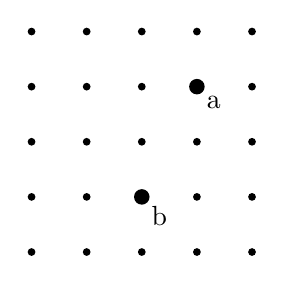
\begin{tikzpicture}[scale=0.7]
  \def\n{5} % Change this value for a grid of different size
  \foreach \x in {1,...,\n} {
    \foreach \y in {1,...,\n} {
      \ifnum\x=3
        \ifnum\y=2
          \fill (\x,\y) circle (4pt);
          \node[anchor=north west] at (\x,\y) {b};
        \else
          \fill (\x,\y) circle (2pt);
        \fi
      \else
        \ifnum\x=4
          \ifnum\y=4
            \fill (\x,\y) circle (4pt);
            \node[anchor=north west] at (\x,\y) {a};
          \else
            \fill (\x,\y) circle (2pt);
          \fi
        \else
          \fill (\x,\y) circle (2pt);
        \fi
      \fi
    }
  }
\end{tikzpicture}
\end{center}
Prove using the Pigeonhole Principle that if we choose $4n-1$ points from an $n \times n$ grid ($n\ge 4$), there must be three chosen points $x, y, z$ such that $x$ dominates $y$ and $y$ dominates $z$. Make sure to state what your pigeons are and what your holes are, as well as how many of each you have.

\textbf{Hint:} If $x, y, z$ lie on the same increasing diagonal as shown in the picture below, then $x$ dominates $y$ and $y$ dominates $z$.
\begin{center}
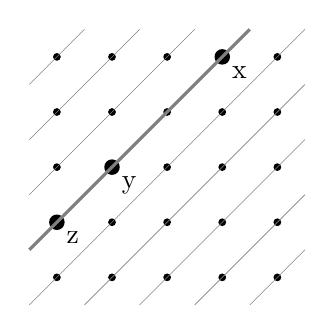
\begin{tikzpicture}[scale=0.7]
  \def\n{5} % Change this value for a grid of different size
  \foreach \x in {1,...,\n} {
    \foreach \y in {1,...,\n} {
      \ifnum\x=4
        \ifnum\y=5
          \fill (\x,\y) circle (4pt);
          \node[anchor=north west] at (\x,\y) {x};
        \else
          \fill (\x,\y) circle (2pt);
        \fi
      \else
        \ifnum\x=2
          \ifnum\y=3
            \fill (\x,\y) circle (4pt);
            \node[anchor=north west] at (\x,\y) {y};
          \else
            \fill (\x,\y) circle (2pt);
          \fi
        \else
          \ifnum\x=1
            \ifnum\y=2
              \fill (\x,\y) circle (4pt);
              \node[anchor=north west] at (\x,\y) {z};
            \else
              \fill (\x,\y) circle (2pt);
            \fi
          \else
            \fill (\x,\y) circle (2pt);
          \fi
        \fi
      \fi
    }
  }

  
  \draw [very thin, gray] (0.5, 4.5) -- (1.5, 5.5);
  \draw [very thin, gray] (0.5, 3.5) -- (2.5, 5.5);
  \draw [very thin, gray] (0.5, 2.5) -- (3.5, 5.5);
  \draw [very thick, gray] (0.5, 1.5) -- (4.5, 5.5);
  \draw [very thin, gray] (0.5, 0.5) -- (5.5, 5.5);%%mid
  \draw [very thin, gray] (1.5, 0.5) -- (5.5, 4.5);
  \draw [very thin, gray] (2.5, 0.5) -- (5.5, 3.5);
  \draw [very thin, gray] (3.5, 0.5) -- (5.5, 2.5);
  \draw [very thin, gray] (4.5, 0.5) -- (5.5, 1.5);

\end{tikzpicture}
\end{center}

\begin{solution} 
An $n \times n$ grid has $2n - 1$ diagonals at $45$ degrees like the ones in the second picture. Let the pigeons be the $4n - 1$ points we choose, and let the holes be the $2n - 1$ diagonals available. By the Pigeonhole Principle, there exists a diagonal at $45$ degrees that contains at least $\lceil \frac{4n - 1}{2n - 1} \rceil = \lceil \frac{4n - 2 + 1}{2n - 1} \rceil = \lceil \frac{4n - 2}{2n - 1} + \frac{1}{2n - 1} \rceil = \lceil 2 + \frac{1}{2n - 1} \rceil = 3$ distinct points we choose. Let $x$ be the point that is the furthest up this diagonal, let $y$ be the point that is the second furthest up this diagonal, and let $z$ be the point that is the third furthest up this diagonal. Therefore, $x$ is strictly above and to the right of $y$, so $x$ dominates $y$. Also, $y$ is strictly above and to the right of $z$, so $y$ dominates $z$.

\smallskip
\textbf{Draft Grading Guidelines [8 points]} 
\begin{gwguidelines}
    \item +1 states that the pigeons are the points we choose
    \item +1 states that we have $4n - 1$ pigeons
    \item +1 states that the holes are the relevant diagonals
    \item +2 states that we have $2n - 1$ holes
    \item +2 uses the Pigeonhole Principle to show that there exists a relevant diagonal with at least $3$ distinct points we choose on it
    \item +1 explains how there being at least $3$ of the points we choose on the same diagonal proves the original statement
\end{gwguidelines}
\end{solution}

\end{document}

